\chapter{Soccer}

One of the favorite games for children is football. The goal of this game is for the player to score as many goals as possible. If he misses, it's game over.

\begin{figure}[H]
   \centering
   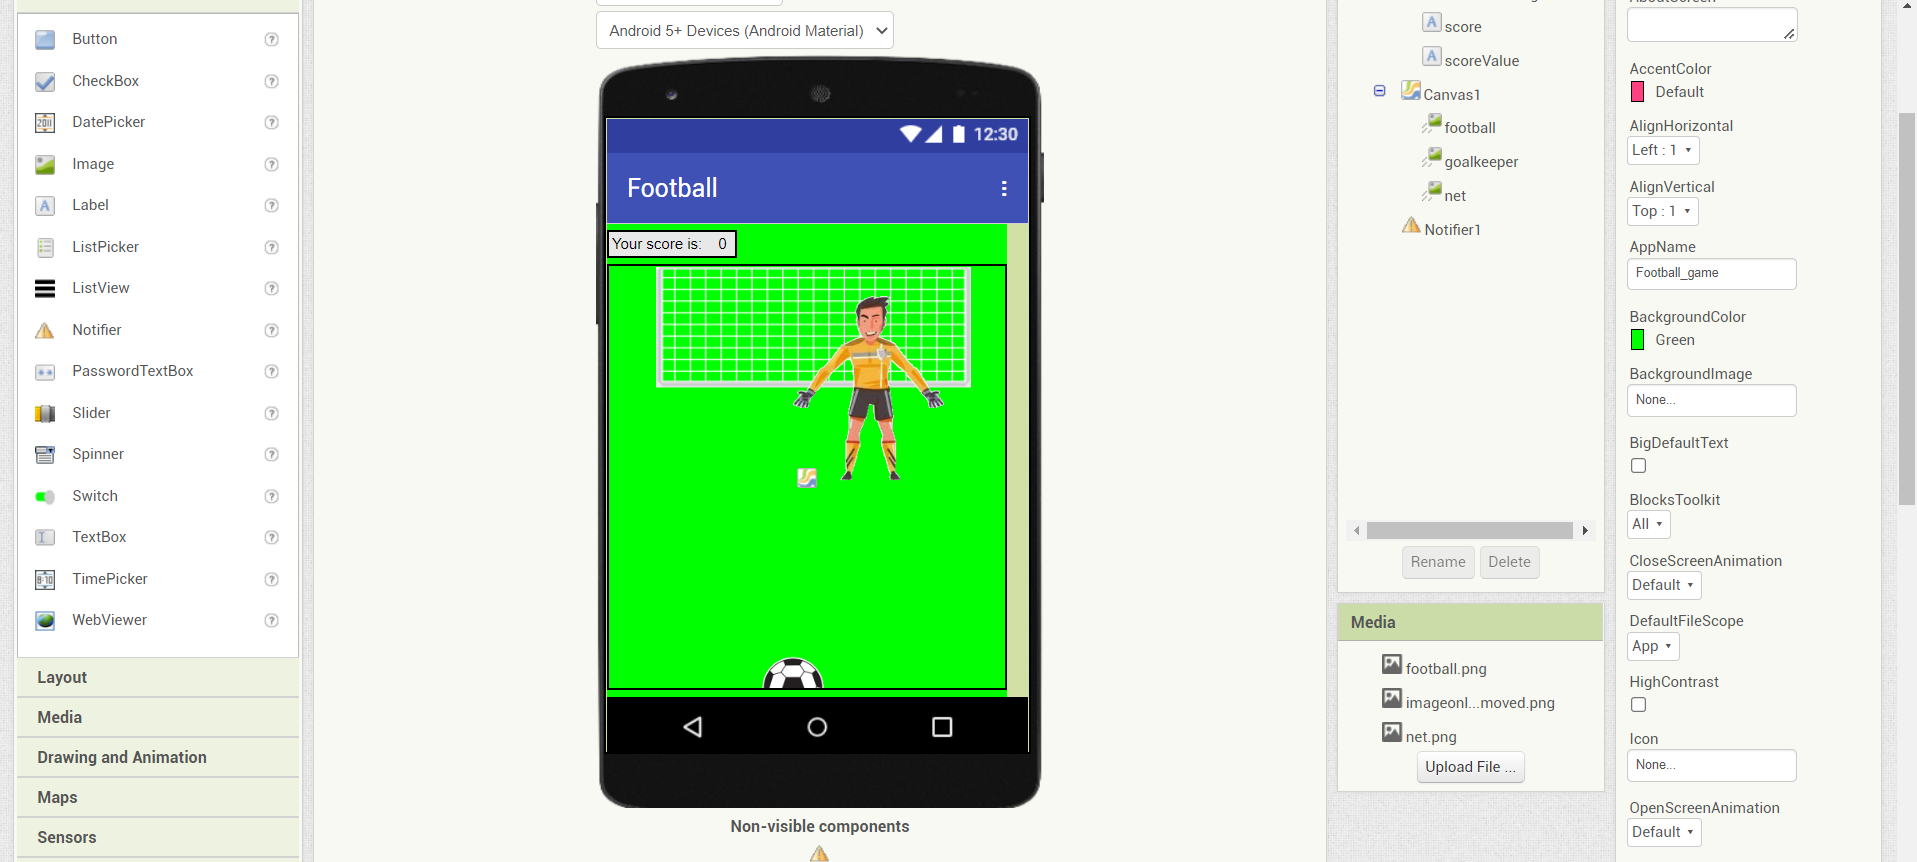
\includegraphics[width=1.0\linewidth,height=0.5\linewidth]{fig110001.png}
   \caption{Football}
\label{fig110001}
\end{figure}

\section{Creating Game Design}
The first step of creating this game is adding all the components that will be programmed. The color of the field should be green. For this, the value of the BackgroundColor property should be changed to green.

\begin{figure}[H]
   \centering
   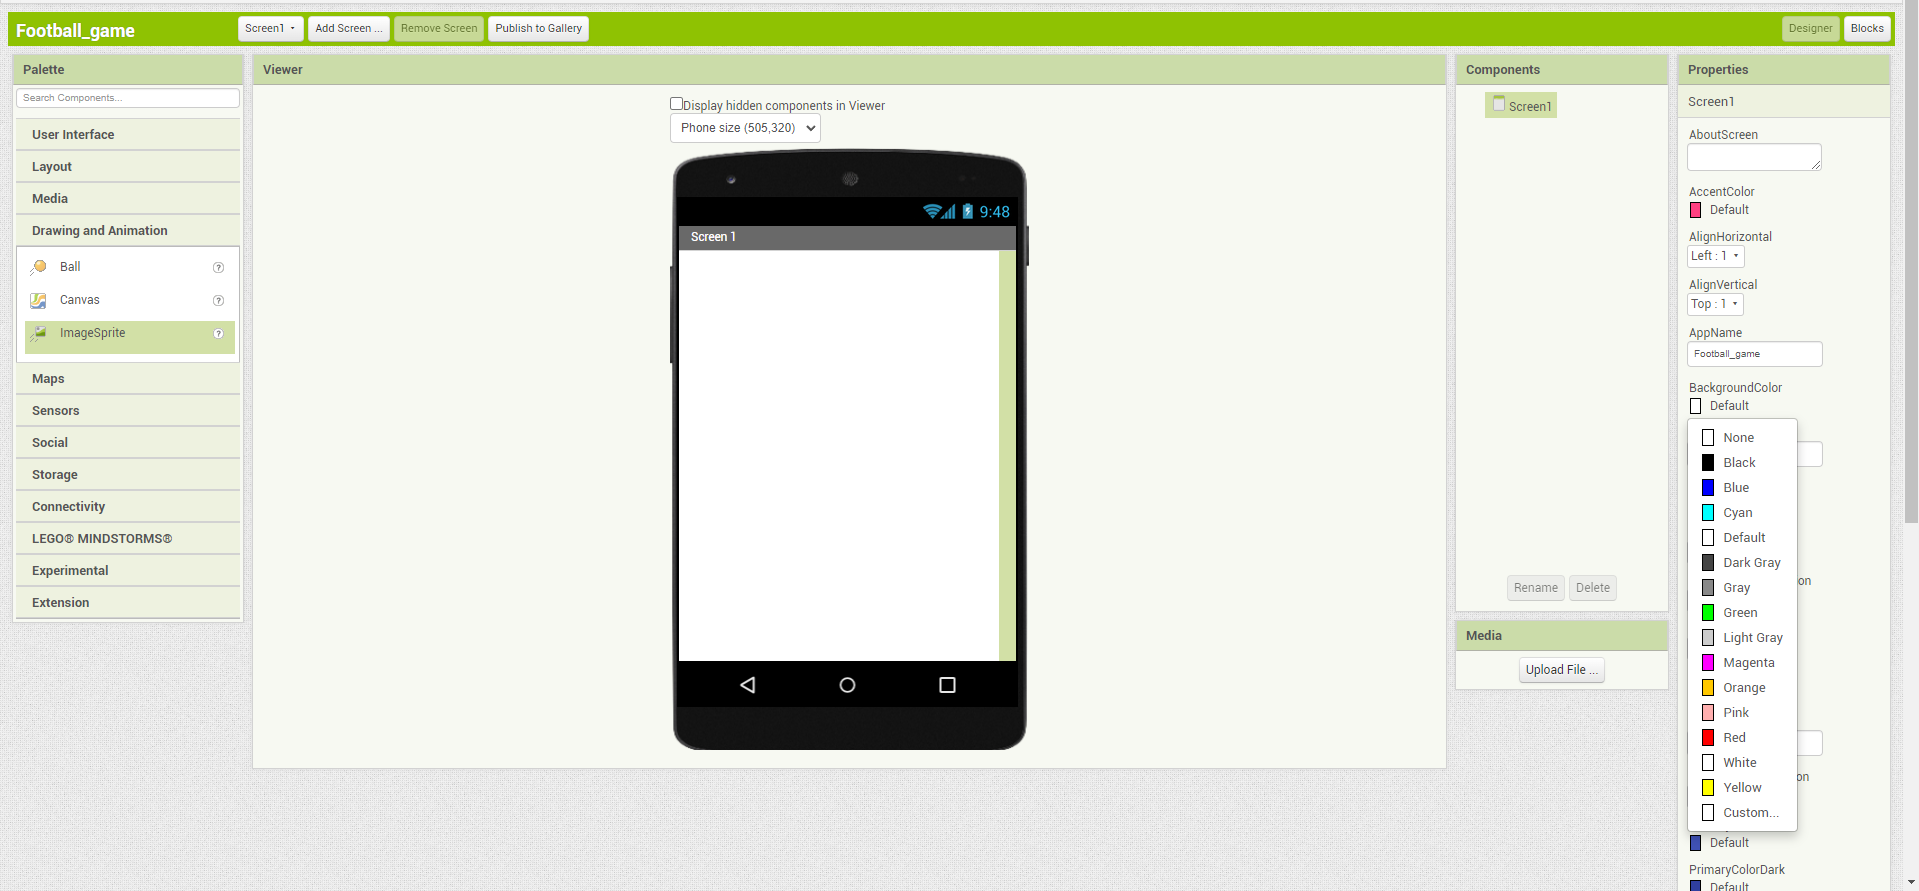
\includegraphics[width=1.0\linewidth,height=0.5\linewidth]{fig110002.png}
   \caption{Change background color}
\label{fig110002}
\end{figure}

One of the most essential tasks in mobile application programming is their interface. To make this game more attractive, you can change the value of the Theme property to Device Default and the name of the Title property to Football.

\begin{figure}[H]
   \centering
   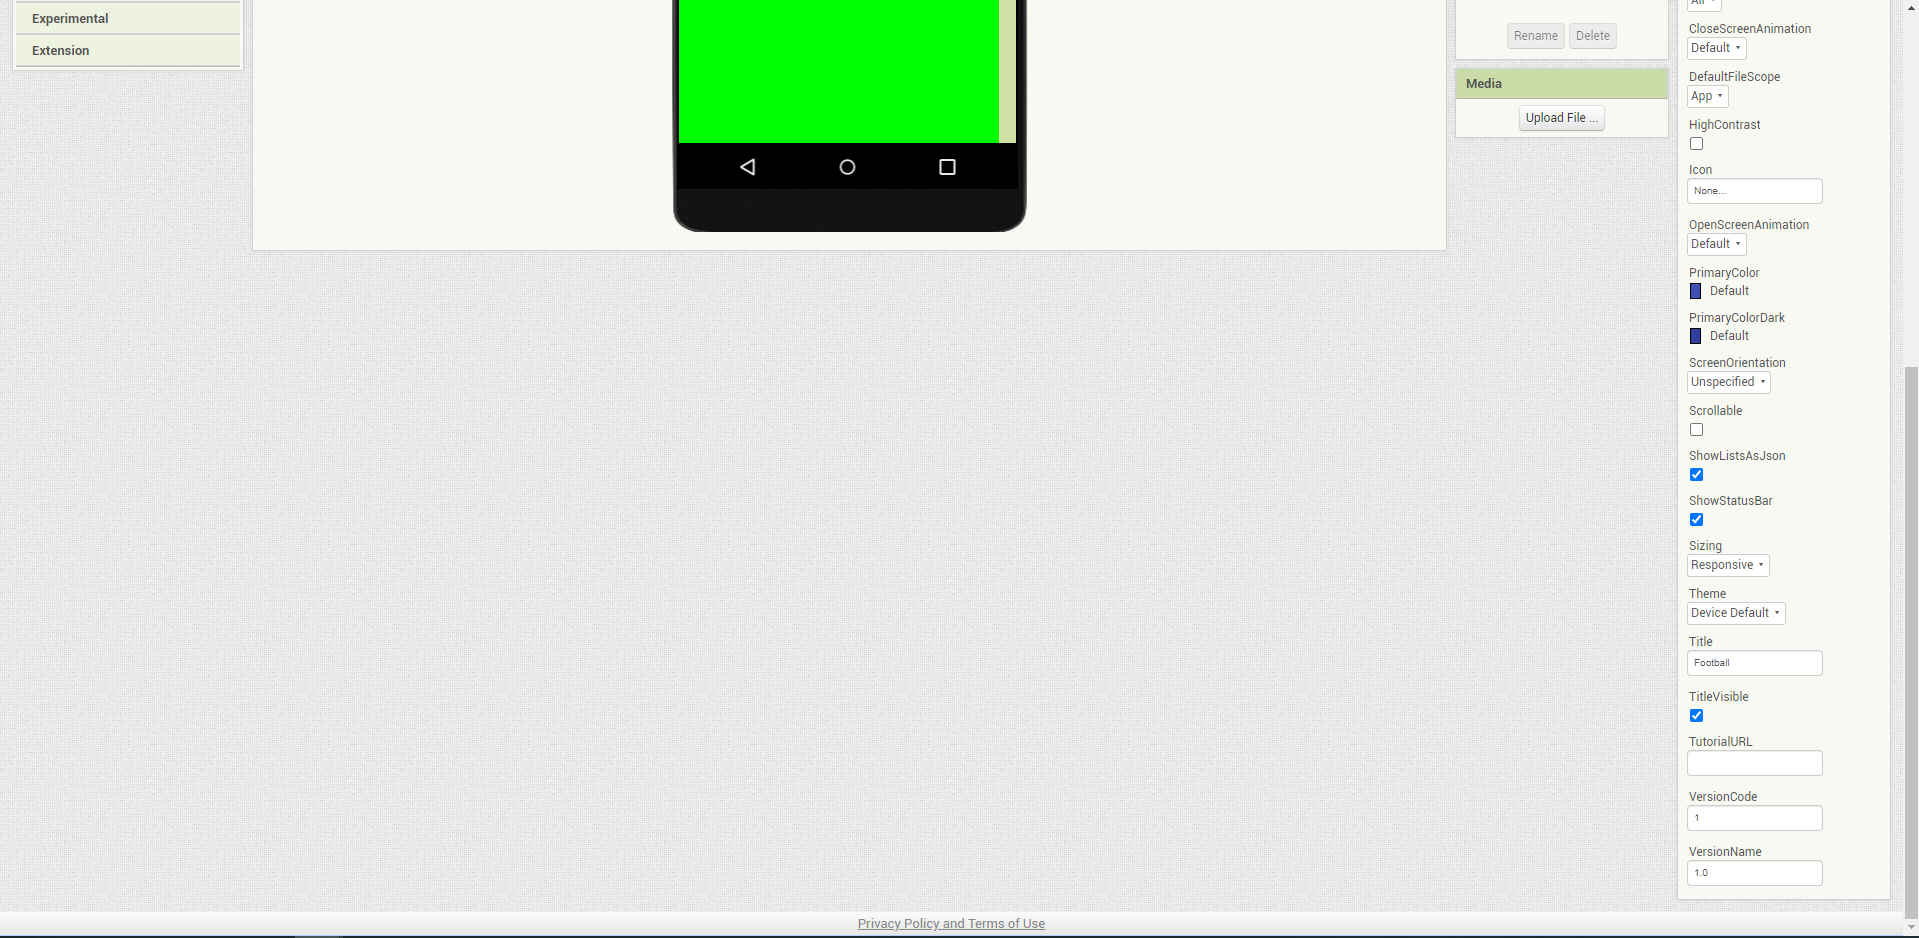
\includegraphics[width=1.0\linewidth,height=0.5\linewidth]{fig110003.png}
   \caption{Change topic}
\label{fig110003}
\end{figure}

For the player to shoot the ball when he touches the screen of his phone and for the goalkeeper to move on the screen, the Canvas element must be added. Its width and height should be the same as on the phone screen. To do this, the Height property values to be Fill parent... The Width property value is the same. This element should blend in with the background color. For this purpose, the value of the BackgroundColor property must be changed.

\begin{figure}[H]
   \centering
   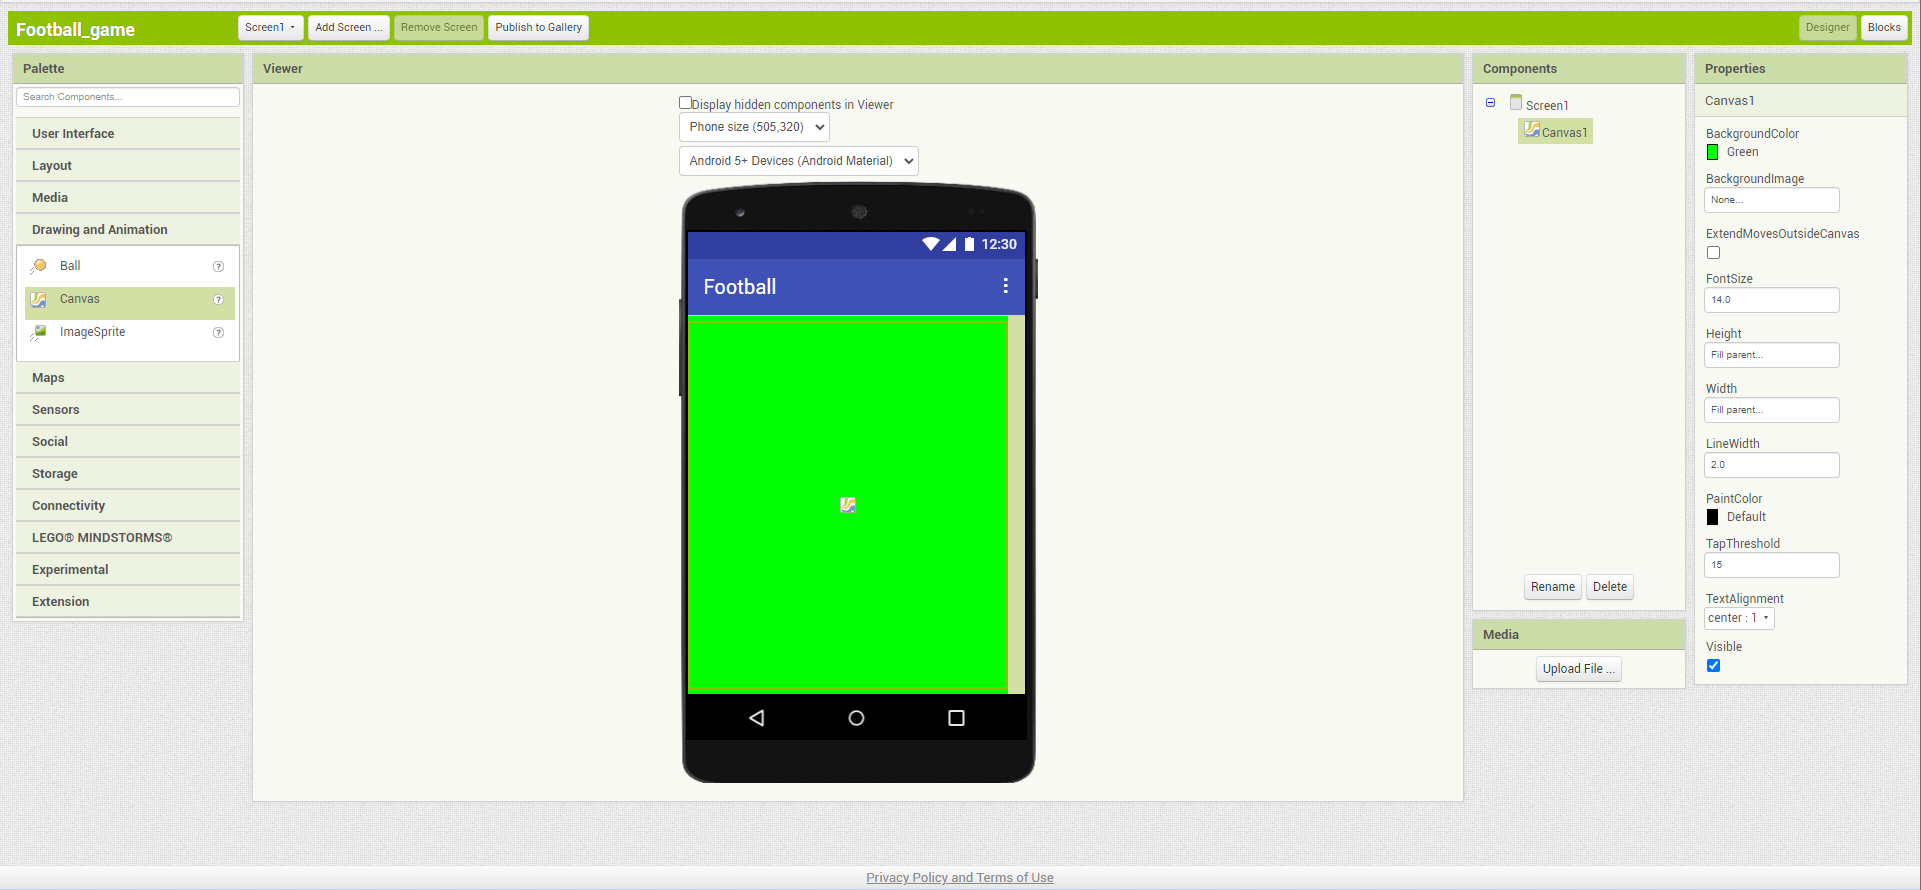
\includegraphics[width=1.0\linewidth,height=0.5\linewidth]{fig110004.png}
   \caption{The Canvas Element}
\label{fig110004}
\end{figure}

Three ImageSprite elements should be added for the net, goalkeeper, and ball. They can be renamed to make it clear which element is for what. Images of these elements can be used, freely licensed for non-commercial use.

\begin{figure}[H]
   \centering
   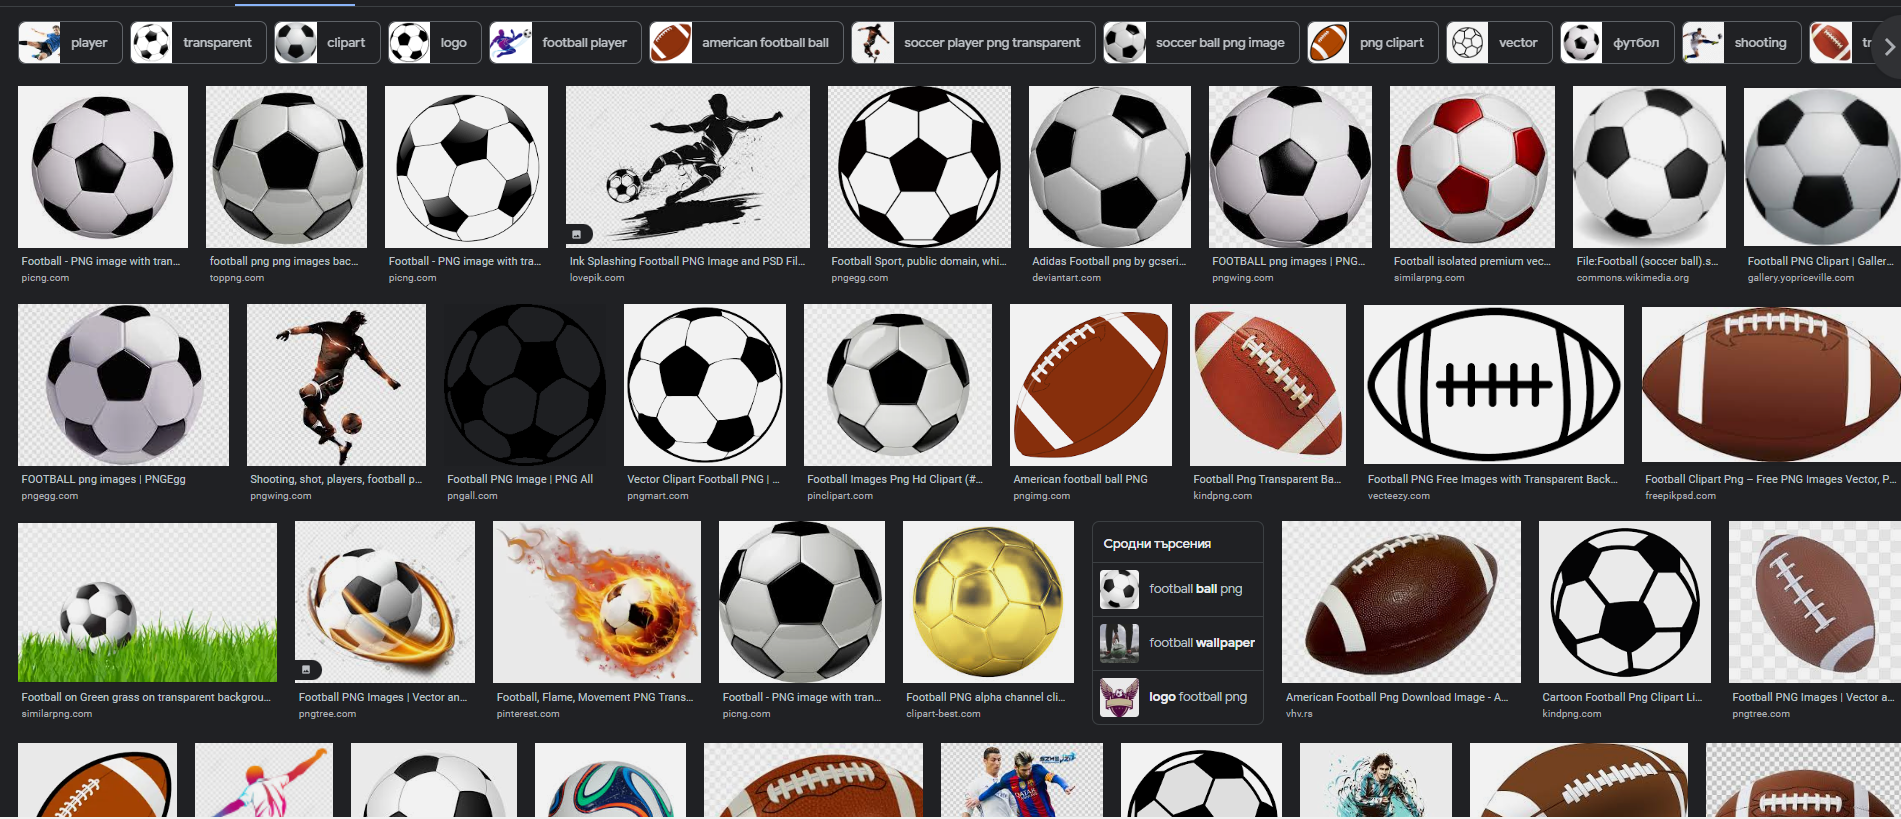
\includegraphics[width=1.0\linewidth,height=0.5\linewidth]{fig110005.png}
   \caption{Image of a soccer ball}
\label{fig110005}
\end{figure}

Once the images are available, they should be placed on the appropriate ImageSprite elements, and the height, width, and position properties should be changed. This means they need to scale to the phone screen. The end result should look like this:

\begin{figure}[H]
   \centering
   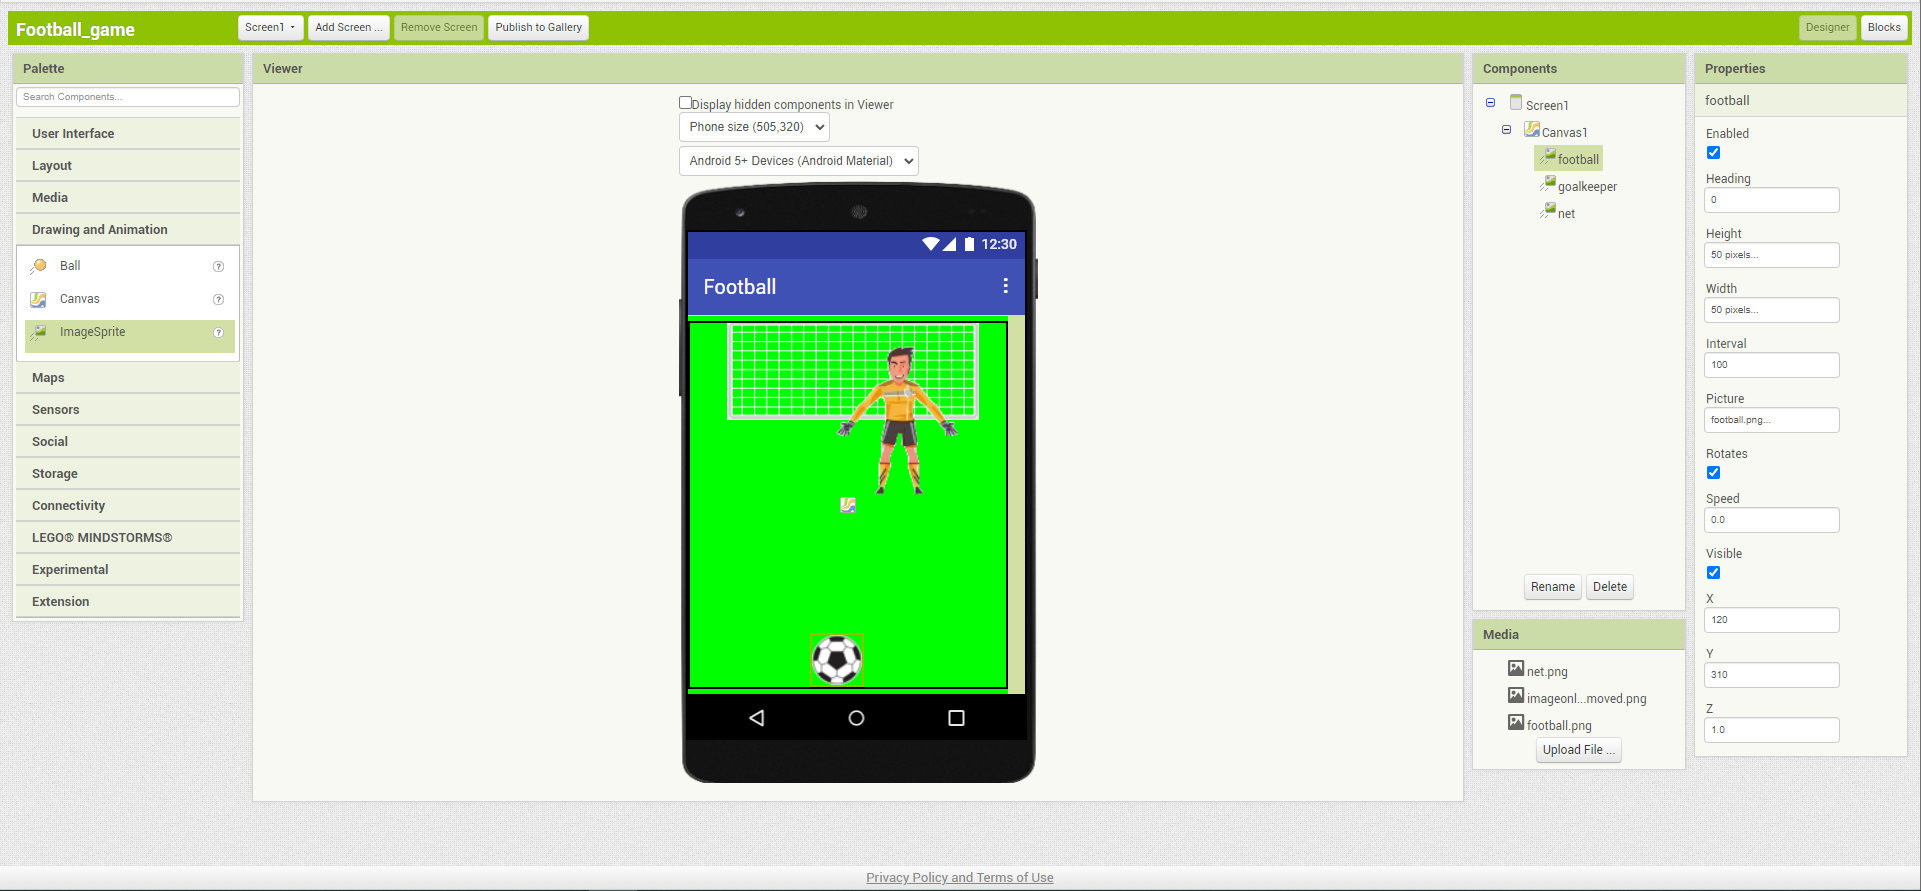
\includegraphics[width=1.0\linewidth,height=0.5\linewidth]{fig110006.png}
   \caption{Game Design}
\label{fig110006}
\end{figure}

In addition to these elements, a place where the result will be written must be added. A HorizontalArrangement element must be added from the Layout element group so that two Label elements can be placed inside it. One will be for the result message, and the second for the result value. This means that the property value for the first label will be "Your score is: " and for the second - "0". Renaming elements to make them easier to program is a good practice. In a later stage of the game, the element "Notifier" will be needed. It is from a group of hidden elements.

\begin{figure}[H]
   \centering
   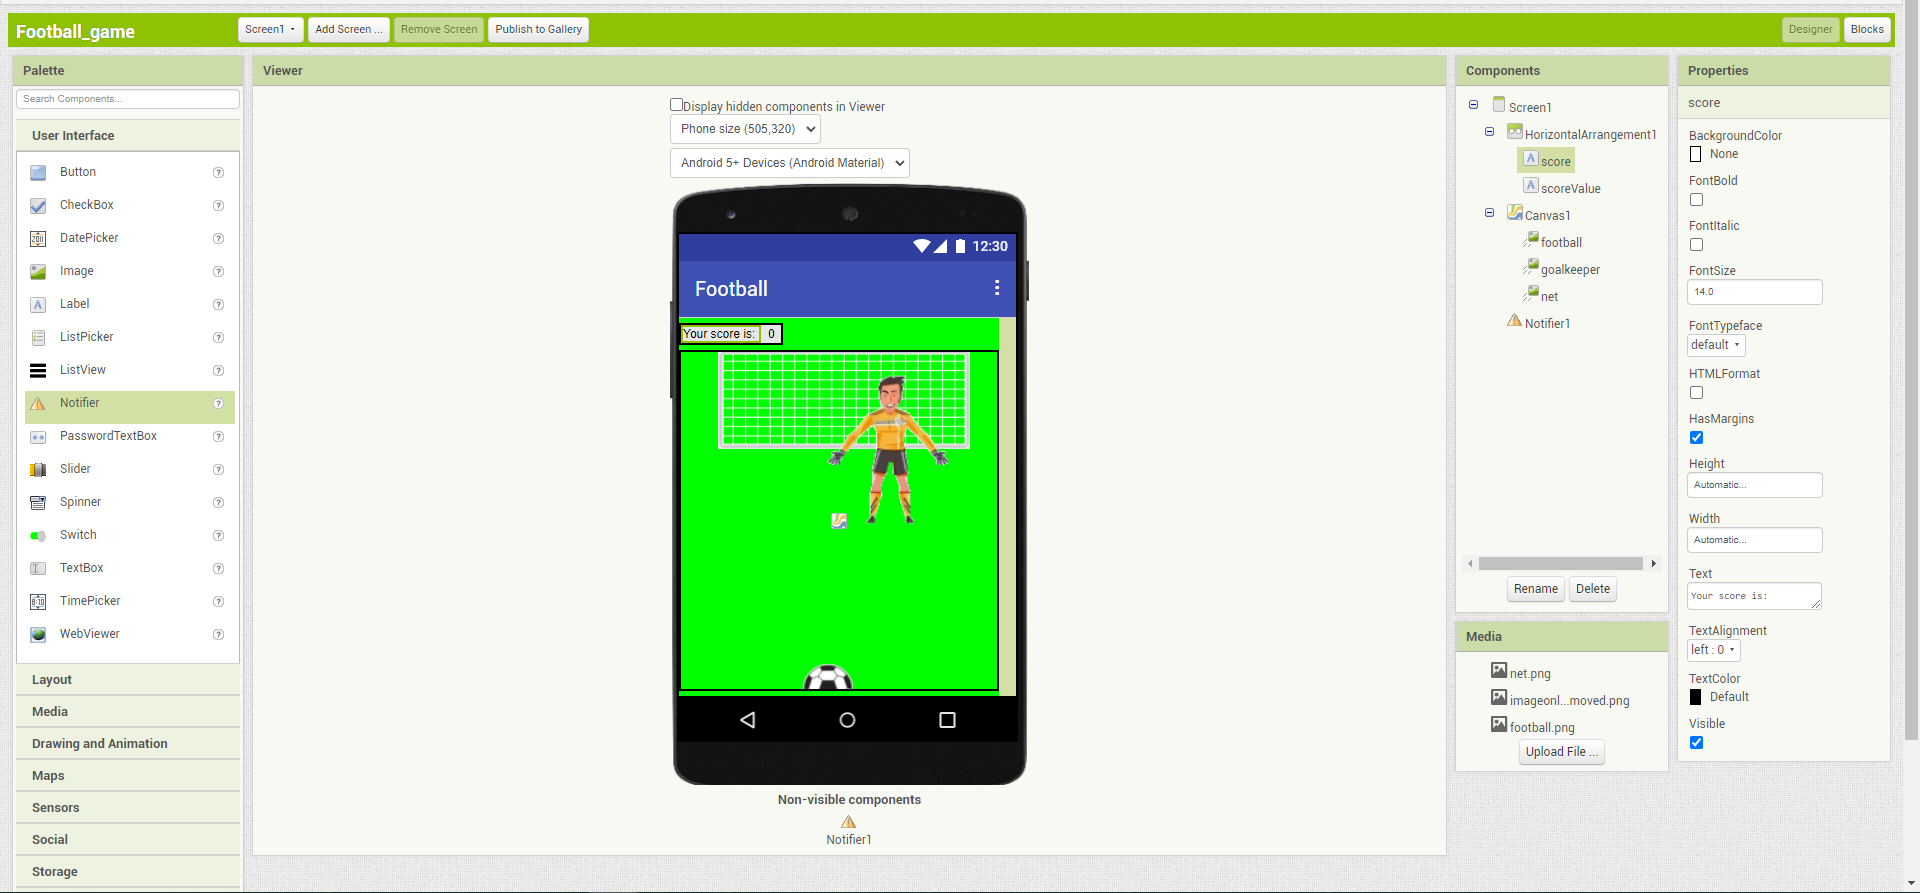
\includegraphics[width=1.0\linewidth,height=0.5\linewidth]{fig110007.png}
   \caption{All Game Elements}
\label{fig110007}
\end{figure}

\section{Programming}
Necessary instructions should also be added to the items for the game. For this purpose, switching to the other view is required, which is for adding the instructions.

The first instructions will be for the goalkeeper. It will move left and right. Its purpose is to keep the goal from scoring. When the game starts, the goalkeeper must start moving. This means adding the when Screen1.Initialize statement found in the Screen1 element. Inside this event, two instructions should be placed in the goalkeeper element. One instruction is to set a value to the Interval property, which specifies how many milliseconds this character's position will change. The second instruction sets a value to the Speed property responsible for the character's movement.

One more event should be added - when the goalkeeper.EdgeReached. The instructions from this event will be executed when the goalkeeper touches the edge of the screen. When this happens, the instruction goalkeeper. The bounce edge is called, and the value set gets the edge.

\begin{figure}[H]
   \centering
   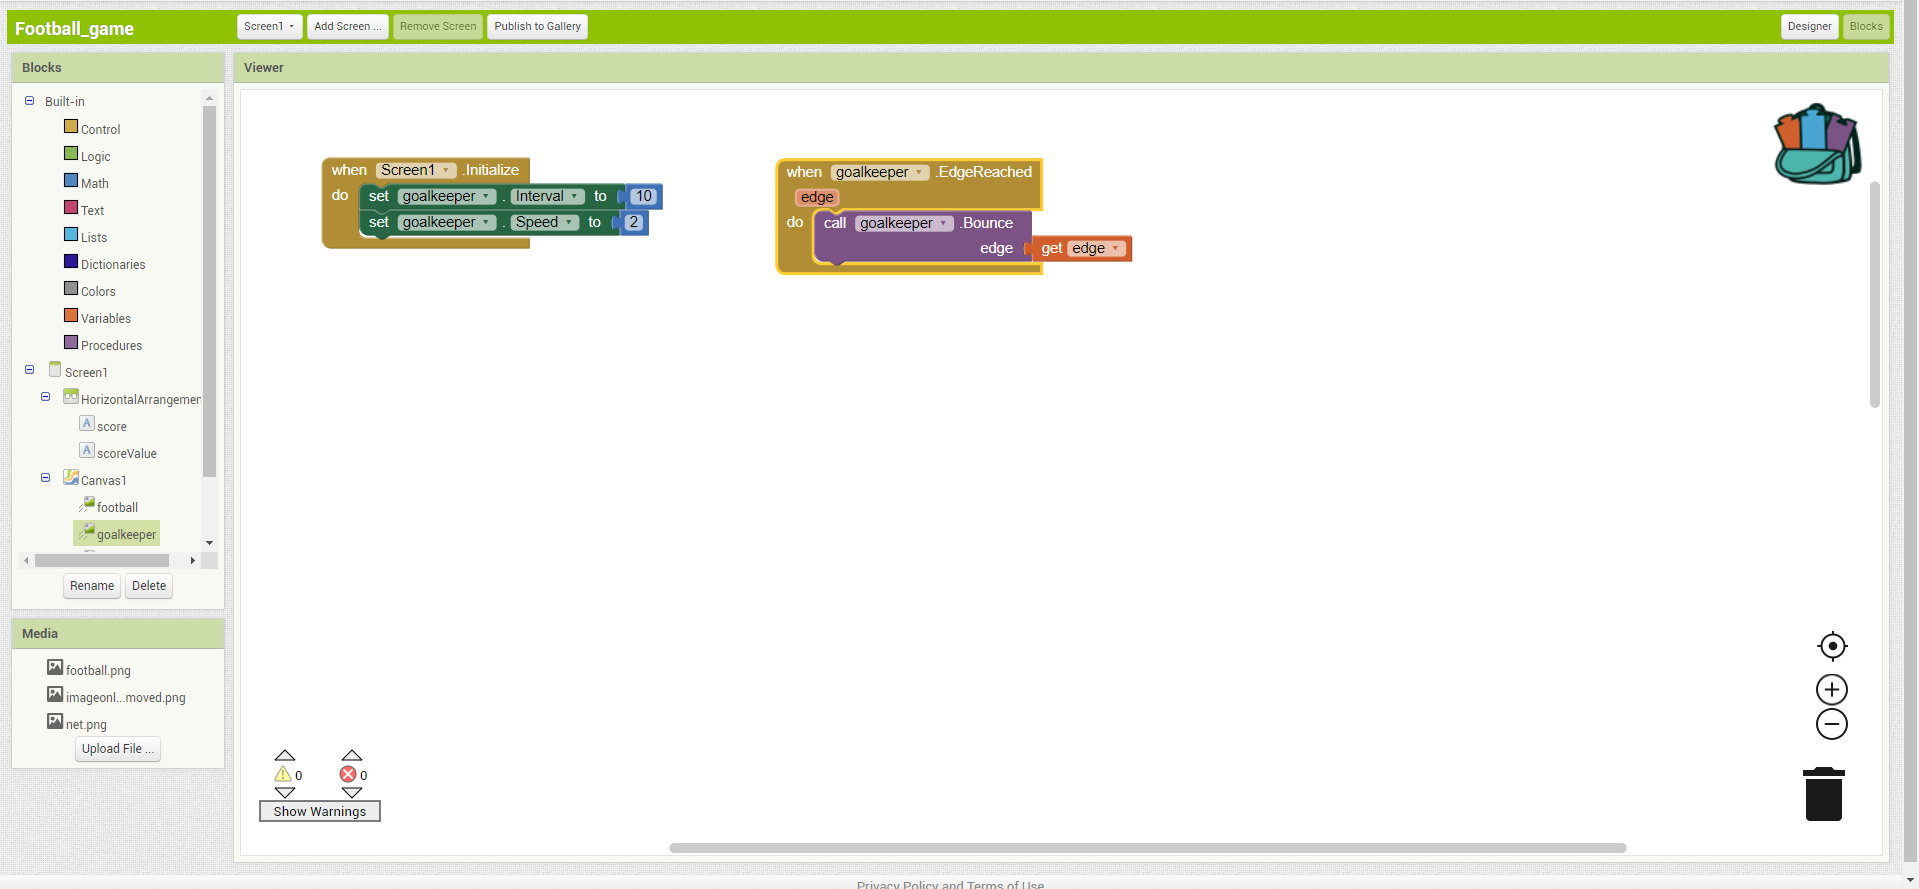
\includegraphics[width=1.0\linewidth,height=0.5\linewidth]{fig110008.png}
   \caption{Goalkeeper Movement}
\label{fig110008}
\end{figure}

When the game starts, it is noticed that the goalkeeper turns with his head down. This can be changed by unchecking the Rotates property.

\begin{figure}[H]
   \centering
   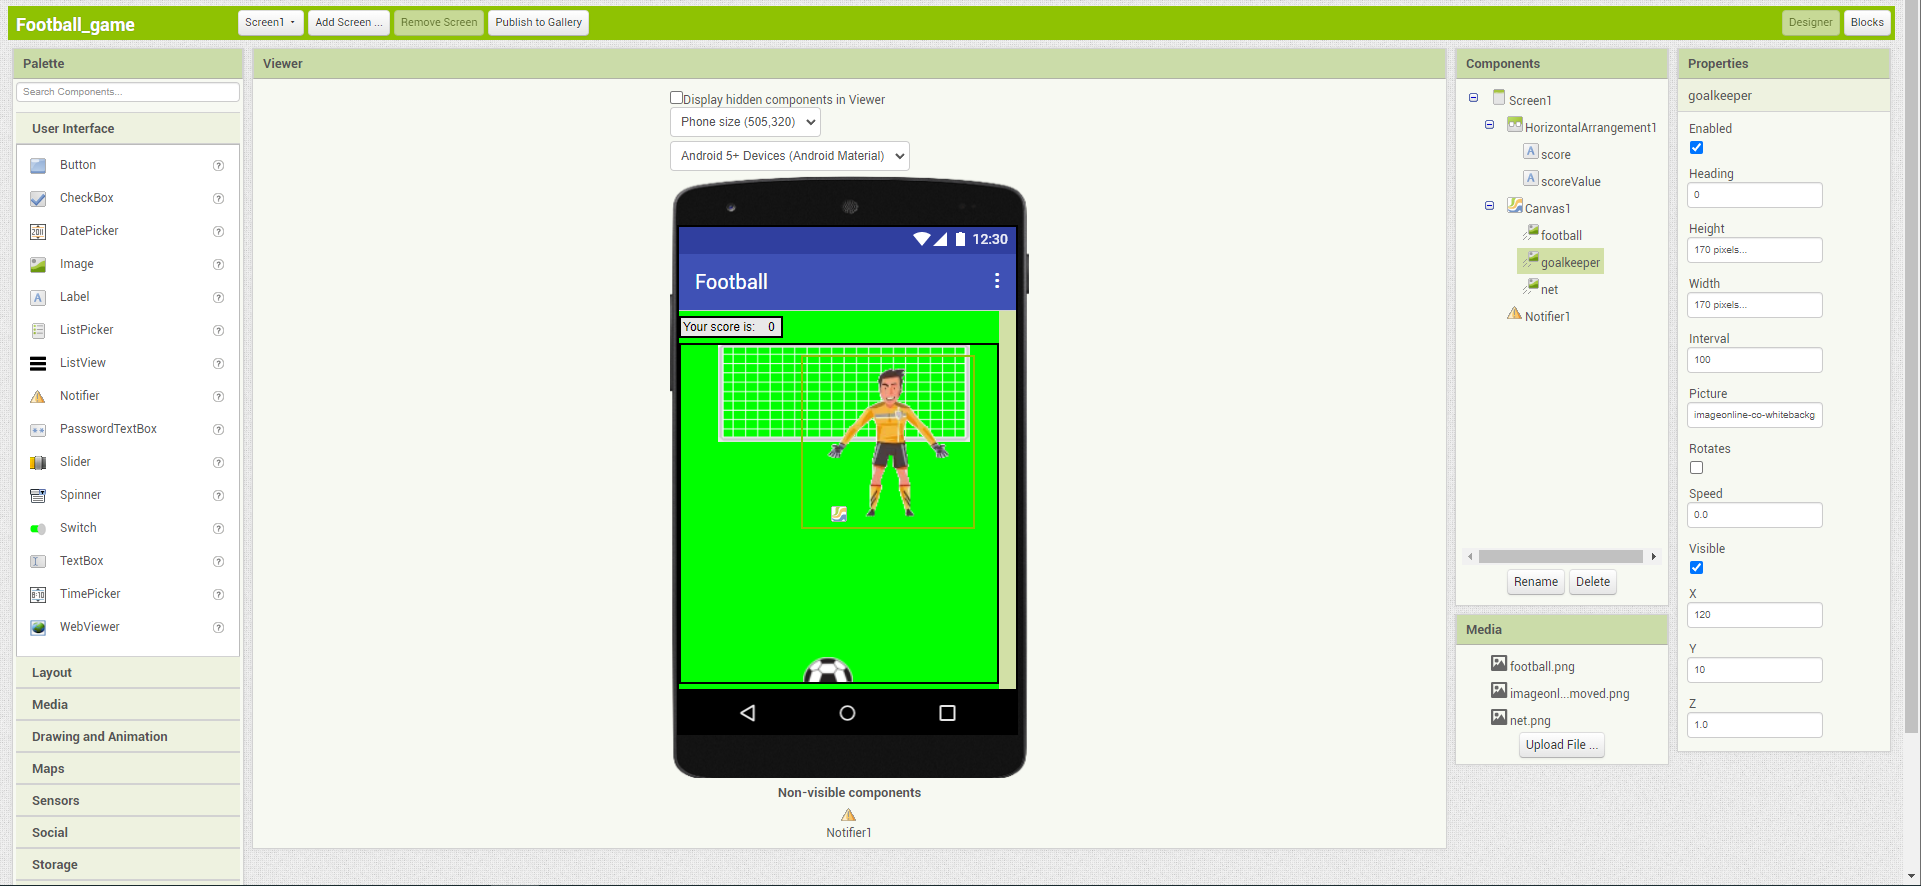
\includegraphics[width=1.0\linewidth,height=0.5\linewidth]{fig110009.png}
   \caption{Stopping goalkeeper rotation}
\label{fig110009}
\end{figure}

Instructions should be added so that when the player drags the ball, it moves. First, when football. A Flug event needs to be added. Similarly, Interval and Speed values should be set for the goalkeeper. The value of the Interval property should be 10, and that of the Speed should be 20. In addition to the movement, the angle at which the ball will move should also be set. For this purpose, a value must be charged for the Heading property from the get-heading event.

\begin{figure}[H]
   \centering
   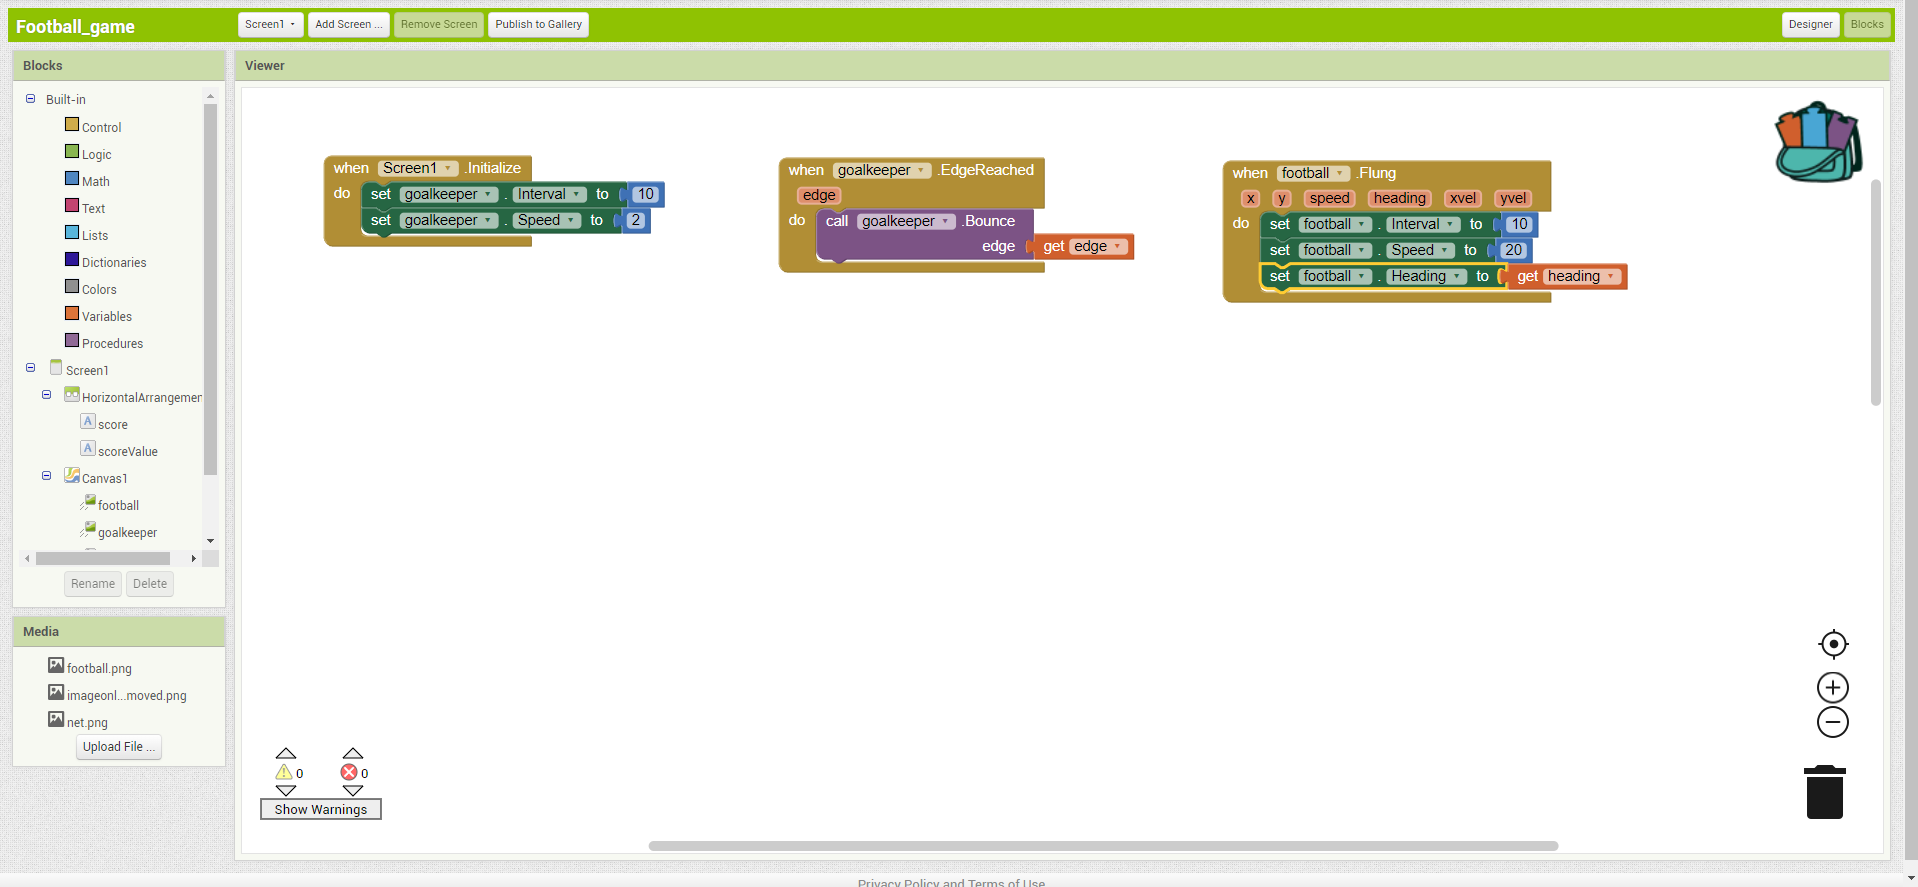
\includegraphics[width=1.0\linewidth,height=0.5\linewidth]{fig110010.png}
   \caption{Ball Movement}
\label{fig110010}
\end{figure}

In the last phase of the game, what happens when the ball touches the net and when it touches the goalkeeper must be programmed. According to the game's rules, when the ball touches the net, the score increases by 1, and when it touches the goalkeeper, the game ends. This means that a variable must be created to store the result of the game. The initial value of this variable is 0.

The event that is needed is when football.CollidedWith. Two checks must be added inside this event - whether the ball touched the net and whether the ball touched the goalkeeper.

\begin{figure}[H]
   \centering
   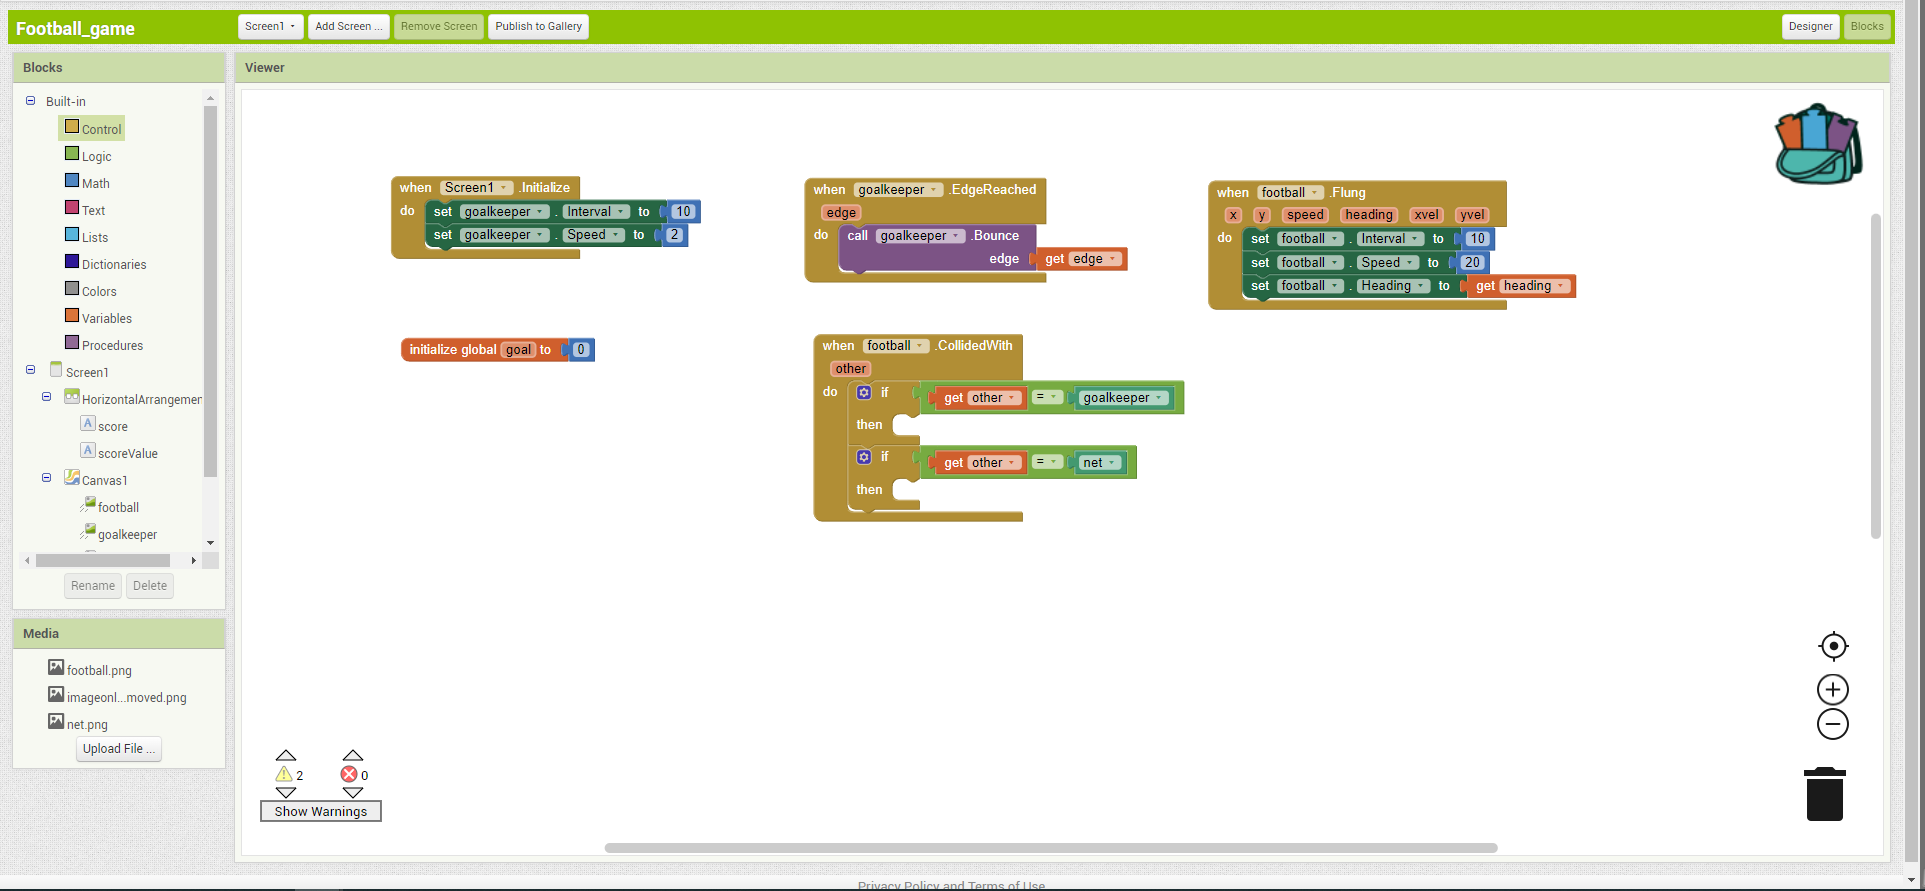
\includegraphics[width=1.0\linewidth,height=0.5\linewidth]{fig110011.png}
   \caption{Adding the checks}
\label{fig110011}
\end{figure}

When the ball touches the goalkeeper, the game must end. In the language of the instructions, some of the properties of the ball should be changed, and a message should be displayed that the game is over. The first ball property to modify is Enabled to false. That means it won't move. Its position should be changed. The values for the coordinates are x=120, y=320, and z=1. The Speed property should be changed to 0.

To display a dialog message, an instruction is added from the Notifier1 element, ShowMessageDialog. It should have the following fields - message="Game over" and title, which consists of the score. Text and scoreValue.Text and the last one is buttonText="Restart game". When the game is over, the variable's initial value, which is 0, must be returned to the scoreValue text field, which is also 0. Remember to change the Enabled value of the ball to true, so it can be played again. Moves the ball.

\begin{figure}[H]
   \centering
   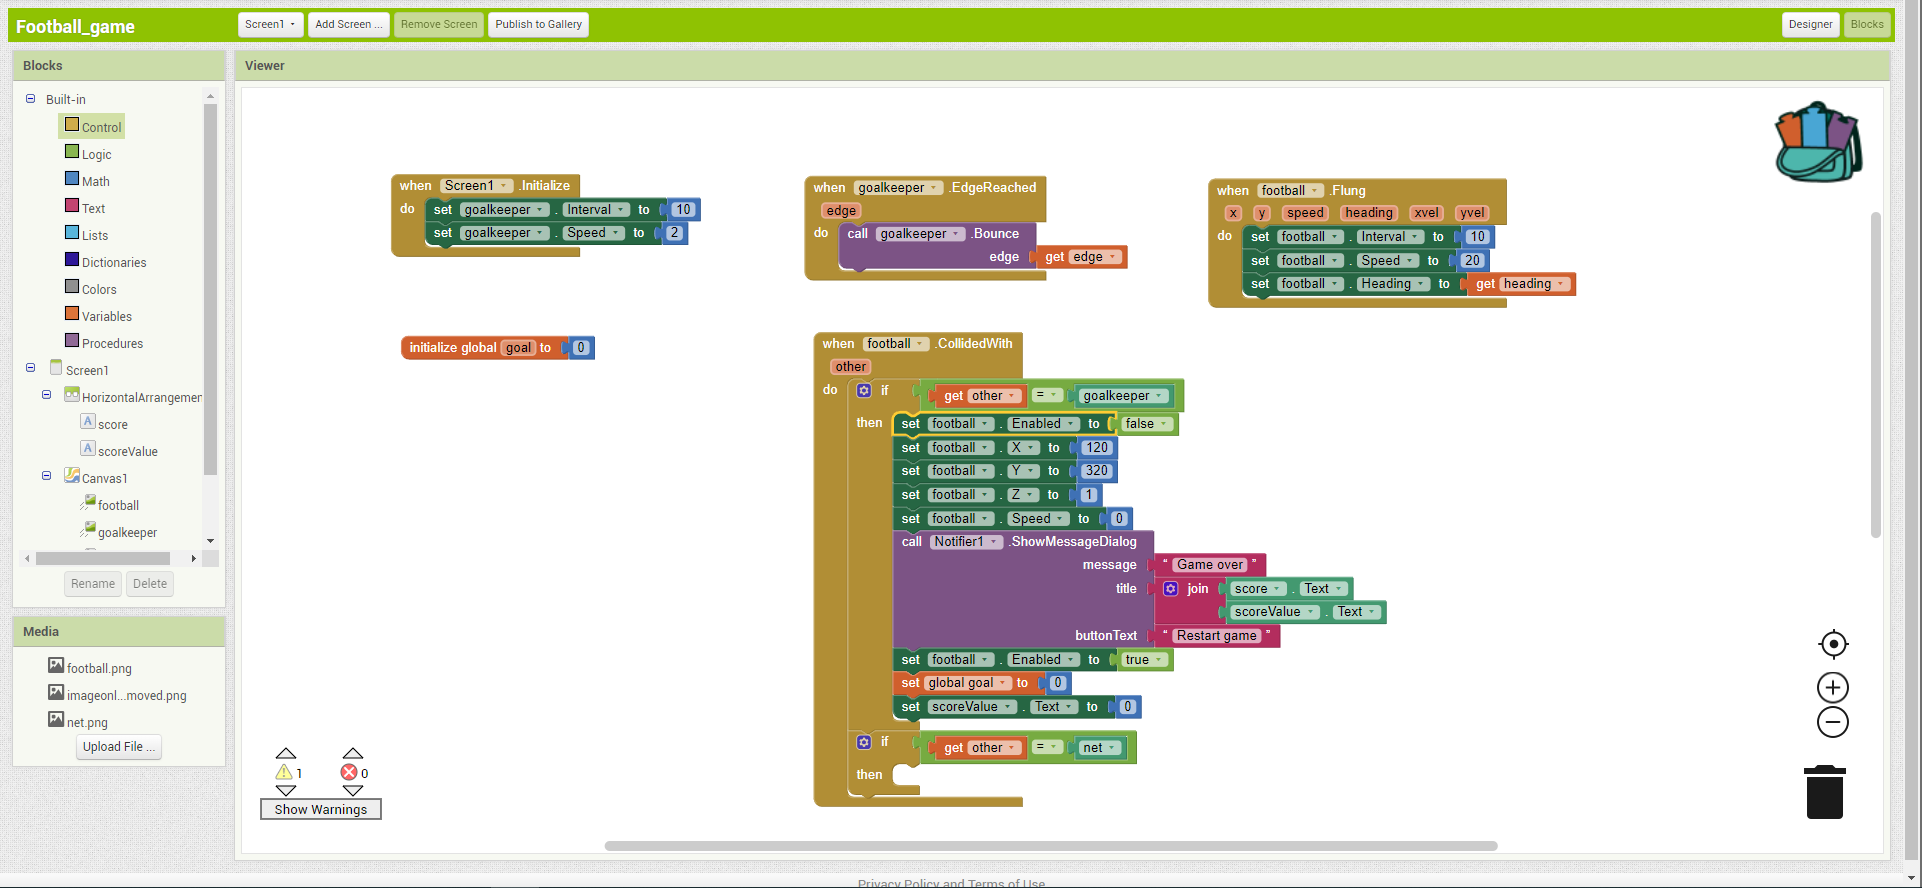
\includegraphics[width=1.0\linewidth,height=0.5\linewidth]{fig110012.png}
   \caption{When the ball touches the goalkeeper}
\label{fig110012}
\end{figure}

When the ball touches the net, the instructions are basically the same. First, the position of the ball must be changed. The difference is that the variable must be incremented, and the new result displayed.

\begin{figure}[H]
   \centering
   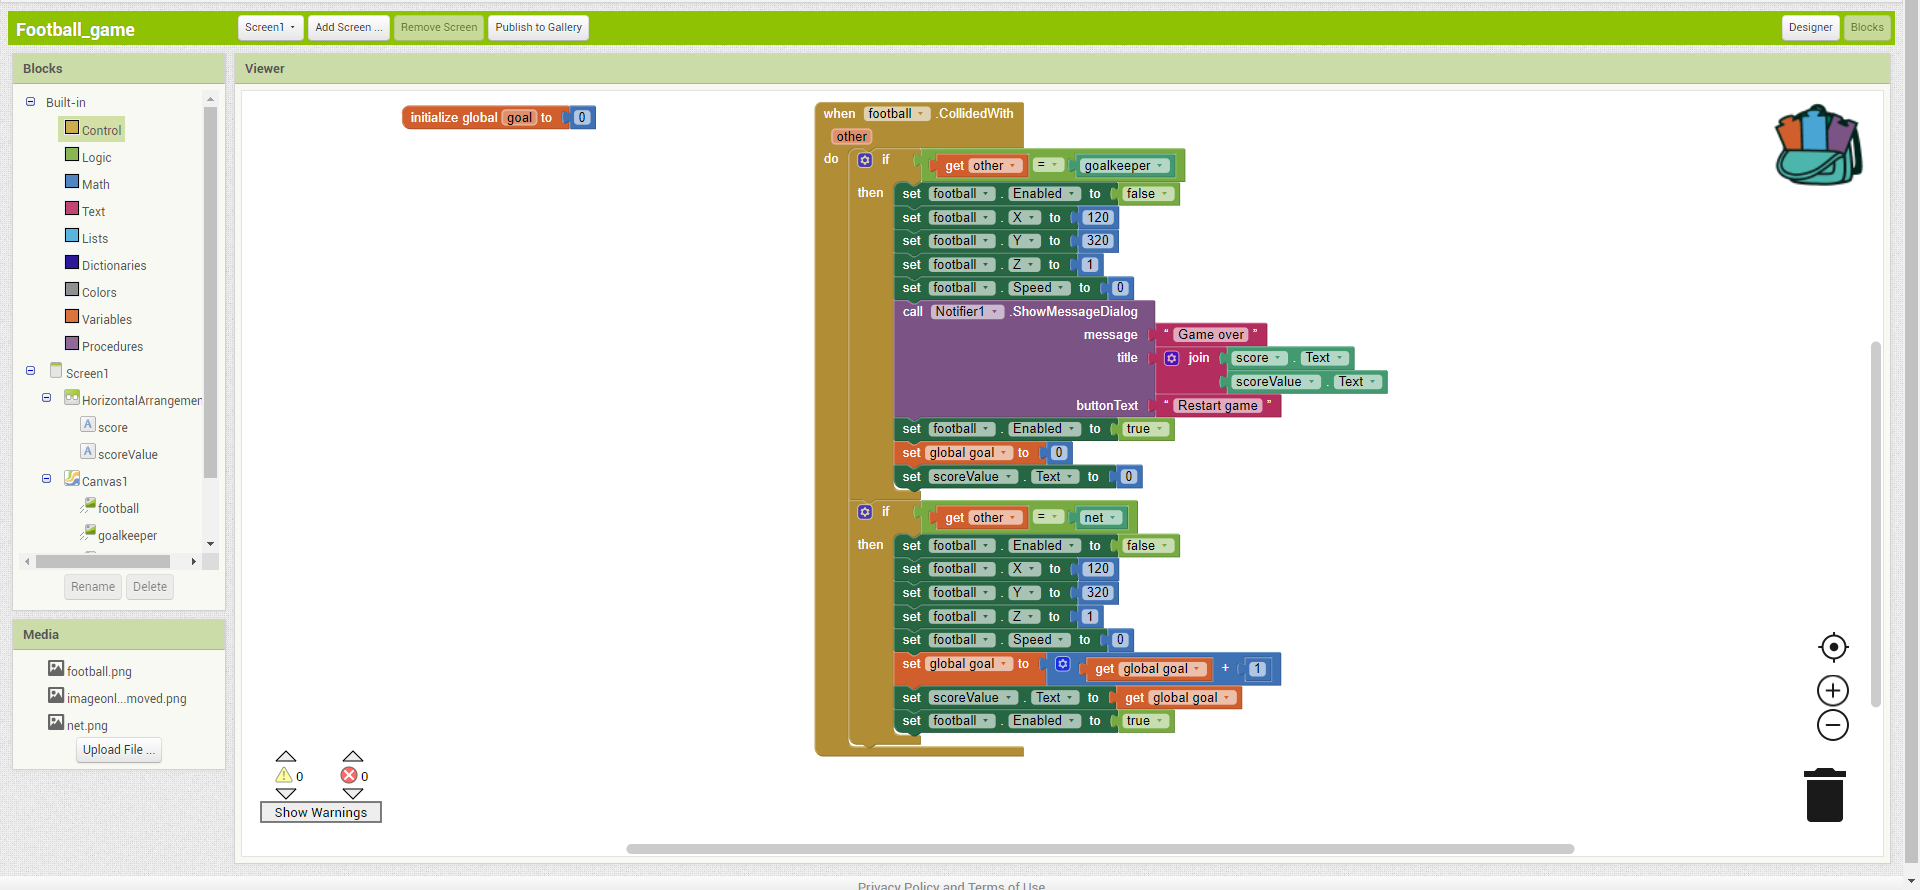
\includegraphics[width=1.0\linewidth,height=0.5\linewidth]{fig110013.png}
   \caption{When the ball hits the net}
\label{fig110013}
\end{figure}

The game is ready. You can compete with your friends to see who is better at scoring goals.
